\section{Machine Learning}


\subsection{Introduction}

Machine Learning differs from traditional programming, we want to model a function to predict data or patterns. Machine Learning has many applications in multiple fields. Since we are using data is important to notice that those can have biases like people. Some biases related to people can be confirmation, falalcy of centrality or survivorship.

\vspace{10pt}

ML as said has many applications, some can be:
\begin{enumerate}
    \item Image and object recognition
    \item Videogames
    \item Sound generation and recognition
    \item Art and style imitation
    \item Predictions
\end{enumerate}

\vspace{10pt}

Many algorithms exist for those tasks but all of them are made from three main components:
\begin{enumerate}
    \item \textbf{Representation} \ra Space of models
    \item \textbf{Evaluation} \ra How to assess which model is better for a certain task
    \item \textbf{Optimization} \ra How to improve the model
\end{enumerate}

Optimizing a model means finding the best parameters and hyperparameters, we can do it via:
\begin{itemize}
    \item Combinatorial optimization
    \item Convex optimization
    \item Constrained optimization
\end{itemize}

\vspace{10pt}

Different tasks require different kind of learning:

\begin{itemize}
    \item \textbf{Supervised/Inductive} \ra We have the labels of the training data
    \item \textbf{Unsupervised} \ra We don't have the labels in the training data
    \item \textbf{Semi-supervised} \ra Mix of the previous two
    \item \textbf{Reinforcement} \ra We want to maximize a reward function after performing some actions
\end{itemize}

More specifically we will study the first one

\vspace{10pt}

\textbf{Supervised} \ra We have many examples of data, we want to find the function that describes best their distribution. We can do classification, regression or estimating probabilities. The core idea is that we want to fit a curve that discriminates between classes or that fit at best a scatterplot. Since we are estimating we will have for sure a certain degree of errors, that is called the \textbf{bias}. Bias can also be positive if is used in a smart way, if we have knowledge about something we can use it to avoid useless steps.

\vspace{10pt}

As we know in the 1-D case a math function is on the form of 

\begin{equation}
    y = f(x)
\end{equation}

And if we open $f(x)$

\begin{equation}
    f(x) = ax + b
\end{equation}

This is the most basic linear case. We want to estimate the parameters a and b to fit the data in the best way. The core idea is to reduce as much uncertainty as possible.

\hrule

\subsection{Machine Learning tribes}

Machine learning implies that the machine will learn something, there are different approaches for that. They can be applied to different tasks for better performances.

\begin{enumerate}
    \item \textbf{Symbolism} \ra Fill gaps in existing knowledge
    \item \textbf{Connectionism} \ra Emulate the brain
    \item \textbf{Evolutionary Computation} \ra Simulate evolution
    \item \textbf{Statistical Learning} \ra Reduce uncertainty
    \item \textbf{Analogy Modelling} \ra Check for similarities between old and new
\end{enumerate}

\begin{table}[h!]
\centering
\begin{tabular}{|l|l|l|}
\hline
\textbf{Tribe} & \textbf{Origins} & \textbf{Master Algorithm} \\ \hline
Symbolists & Logic, Philosophy & Inverse Deduction \\ \hline
Connectionists & Neuroscience & Backpropagation \\ \hline
Evolutionaries & Evolutionary Biology & Genetic Programming \\ \hline
Bayesians & Statistics, Probability & Inference \\ \hline
Analogizers & Psychology & Support Vector Machines (SVM) \\ \hline
\end{tabular}
\end{table}

\textbf{Symbolists}:
\begin{itemize}
    \item Logic programming
    \item Expert systems
    \item Decision trees
    \item Functional programming
\end{itemize}

\textbf{Connectionists}:
\begin{itemize}
    \item Perceptron
    \item MLP
    \item DNN
    \item Hopfield networks
    \item Boltzmann networks
\end{itemize}

\textbf{Evolutionary}:
\begin{itemize}
    \item Genetic algorithms
    \item Genetic programming
    \item Ant Colony optimization
    \item Particle Swarm optimization
\end{itemize}

\textbf{Bayesians}:
\begin{itemize}
    \item Bayesian classifiers
    \item Bayesian Belief networks
    \item Markov models
\end{itemize}

\textbf{Analogizers}:
\begin{itemize}
    \item KNN
    \item Self-organization
    \item SVM
\end{itemize}

If we cross together the tribes and the components seen in the previous class we can see that:

\begin{itemize}
    \item \textbf{Representation}
    \begin{itemize}
        \item Probabilistic Logic
        \item Each rule has a weight
    \end{itemize}
    \item \textbf{Evaluation}
    \begin{itemize}
        \item Posterior probability
        \item User defined objective function
    \end{itemize}
    \item \textbf{Optimization}
    \begin{itemize}
        \item Genetic programming
        \item Backpropagation
    \end{itemize}
\end{itemize}


\subsection{Feature Selection}

The most important part of a machine learning model is the dataset, sometimes the data aren't good enough on their own so we must account for that. Some ways are

\begin{itemize}
    \item \textbf{Feature extraction and engineering} \ra extract something from simpler features
    \item \textbf{Feature transformation} \ra modify the features to make them more useful for the model
    \item \textbf{Feature selection} \ra use the most relevant features
\end{itemize}

In this course we will see mainly the third point. When we do \textbf{Feature selection} we aim to reduce the number of inputs variables to a subset that can be equally useful. Simpler models are easier to interpret, the training time is reduced, generalization is enhanced and we remove redundant variables.

\vspace{10pt}

Feature selection is done via 3 main methods:
\begin{itemize}
    \item \textbf{Filter methods} \ra Statistical methods to evaluate the importance of the features, like correlation
    \item \textbf{Wrapper methods} \ra We train a model with subsets of features until we find the best one
    \item \textbf{Embedded methods} \ra During the training of our model the importance of the features is assessed. 
\end{itemize}

\textbf{Filter methods}:
\begin{itemize}
    \item Pearson correlation coefficient
    \item Spearman rank coefficient
    \item ANOVA correlation coefficient
    \item Kendall rank coefficient
    \item Chi-Squared test
    \item Mutual information
\end{itemize}

\vspace{10pt}

Pearson Correlation coefficient, it measures linear correlation:
\begin{equation*}
    \rho_{X,Y} = \frac{\text{cov(X,Y)}}{\sigma_X \sigma_Y}
\end{equation*}

For m samples

\begin{equation*}
r = \frac{\sum_{i=1}^{m} (x_i - \bar{x})(y_i - \bar{y})}
{\sqrt{\sum_{i=1}^{m} (x_i - \bar{x})^2} \; \sqrt{\sum_{i=1}^{m} (y_i - \bar{y})^2}}
\end{equation*}

Spearman rank correlation coefficient, it asses how well the relationship between two variables can be described by a monotonic function

\begin{equation*}
    r_s = \rho_{rg_x,rg_y}= \frac{cov(rg_x,rg_y}{\sigma_{rg_x}\sigma_{rg_y}}
\end{equation*}

\vspace{10pt}

We shouldn't always discard variables with a small score. It depends by case to case

\vspace{10pt}

We can also use \textbf{Mutual information}, this can help finding non-linear dependencies but is harder to estimate than pure correlation.

\vspace{10pt}

Mutual information (continuous and discrete), for non linear and non monotonic relationships

% Caso continuo
\begin{equation*}
I(X_i; y) = \int \int p(x_i, y) \, \log \frac{p(x_i, y)}{p(x_i)\, p(y)} \, dx \, dy
\end{equation*}

% Caso discreto
\begin{equation*}
I(X_i; Y) = \sum_{x_i} \sum_{y} P(X = x_i, Y = y) \, \log \frac{P(X = x_i, Y = y)}{P(X = x_i) \, P(Y = y)}
\end{equation*}

The problem is that mutual information can be inconvenient for feature ranking. To solve the associated problems we can use the \textbf{Maximal information coefficient} that transforms the previous and binds it in [0;1]. We obtain the percent of a variable Y that can be explained by a variable x

\begin{equation*}
\text{MIC}(X, Y) = \max \{\frac{I(x, y)}{\log_2 \min\{ n_x, n_y \}}\}
\end{equation*}

\vspace{10pt}

\textbf{Wrapper methods}

We consider certain subsets of our features, at each iteration we try to find the best combination of those. We can vary which and how many features to consider. The selection process involves evaluate the subsets using a predictive model and using the subset with the best performance.

\vspace{10pt}

The search process can use different strategies:
\begin{itemize}
    \item Methodical
    \item Stochastic
    \item Heuristics
\end{itemize}

\vspace{10pt}

One of the most used is RFE
\begin{enumerate}
    \item The model is fitted on all the predictors
    \item Each predictor is ranked using it's importance to the model
    \item We choose the n top ranked predictors
    \item We find the best number n with the best n features
\end{enumerate}

RFE can encounter problems if it overfit on uninformative features.

\vspace{10pt}

Our training set is used for selecting predictors, fitting the model and evaluating the performance.

To improve RFE we can add \textbf{Cross-validation}

\vspace{10pt}

\textbf{Embedded methods}

This last kind of methods consists in regularizing the model while it's been created. The process consists in adding constraints into the optimization and adding a bias toward lower complexity, so reducing the number of coefficients

\vspace{10pt}

We have two main regularization algorithms:
\begin{enumerate}
    \item Ridge, or L2
    \item Lasso or L1
\end{enumerate}

\vspace{10pt}

Ridge Regression tries to minimize the sum of squared residuals and the slope of the line. This can cause many lower coefficients and can solve for parameters where we do not enough data samples.


\includegraphics{L2.png}

\vspace{10pt}

Lasso Regression on the other hand tries to minimize the magnitudes. It can lead to many zero values in our coefficients set

%\begin{tikzpicture}
%\node[inner sep=0pt] at (0,0) {\pgfimage[width=10cm]{Courses/images/L1.png}};
%\end{tikzpicture}


\includegraphics{L1.png}





\hrule



\subsection{Linear and Logistic Regression}

Today we look at our first algorithms, we start with \textbf{Linear Regression}.

\vspace{10pt}

We want to find a relationship between independent variables and the dependent one. The objective is to make predictions based on the past observations.

\vspace{10pt}

As we know one kind of task for ML models is regression, we want to predict a continuous values. One way is using Linear Regression.

The steps are:
\begin{enumerate}
    \item Use least-squares to fit a line on the data
    \item Calculate the $R^2$
    \item Calculate the p-value for $R^2$
\end{enumerate}

A regression model can be simple or multiple

\begin{equation}
    Y = \beta_0 + \beta_1X_1+ \beta_2X_2+...+\beta_nX_n+\varepsilon
\end{equation}

Where:
\begin{itemize}
    \item Y \ra Model/output
    \item $\beta_0$ \ra Intercept
    \item $\beta_n$ \ra Parameters
    \item $X_n$ \ra Inputs
    \item $\varepsilon$ \ra Residuals
\end{itemize}

\vspace{10pt}

For the simple model we only use the first 2 $\beta$ and the first X

We want to minimize the squared sum of the residuals, this will give us a good model. Since this is a minimization problem on both the parameters we differentiate them getting the following formulas (notes that those are estimations)

\begin{equation}
    \hat{\beta_1} = \frac{\Sigma(X_i-\bar{X})(Y_i-\bar{Y})}{\Sigma(X_i-\bar{X})^2}
\end{equation}

\begin{equation}
    \hat{\beta_0} = \hat{Y} - \hat{\beta_1}\bar{X}
\end{equation}

\vspace{10pt}

As said these are estimations, so we want to evaluate how good they are.

Usually we use $R^2$, it explains how much variation in the output can be explained differently from using just the mean.

\begin{equation}
    R^2 = \frac{SS(mean)- SS(fit)}{SS(mean)}
\end{equation}

Where

\begin{itemize}
    \item SS(mean) or SST \ra $\Sigma(y_i-\bar{y})^2$
    \item SS(fit) or SSE = \ra $\Sigma(y_i-\hat{y_i})^2$
\end{itemize}

\vspace{10pt}

We can also do

\begin{equation}
    R^2=\frac{\text{Var(mean) - Var(fit)}}{\text{Var(mean)}}
\end{equation}

Where

\begin{itemize}
    \item Var(mean) = $\frac{\Sigma(y_i-\bar{y})^2}{n}$ = $\frac{SS(mean)}{n}$
    \item Var(fit) = $\frac{\Sigma(y_i-\hat{y}_i)^2}{n}$ = $\frac{SS(fit)}{n}$
\end{itemize}

\vspace{10pt}

Since bigger models with more features will explain more variability we can use the adjusted $R^2$, it will penalize models with a lot of independent variables

\begin{equation}
    \text{Adjusted }R^2 = 1-\frac{(1-R^2)(N-1)}{N-p-1}
\end{equation}

Where
\begin{itemize}
    \item $R^2$ \ra Current $R^2$
    \item N \ra Samples
    \item p \ra Number of independent variables
\end{itemize}

\vspace{10pt}

After that we can check the p-value for each independent variable to check it's statistical relevance, low p-value means high probability that the variable is useful.

\vspace{10pt}

Another model that we have to look at is \textbf{Logistic Regression}, despite the name is a classifier and not a regressor. We want to make a binary classification (1 or 0) based on our data. Differently from the Linear regression loss function (SSE) here we use MLE (Maximum Likelihood Estimation) to maximize the probability of being right.

\vspace{10pt}

Usually our decision is like this

\begin{equation}
    \begin{cases}
        \text{1 \hspace{10pt} if True} \\
        \text{0 \hspace{10pt} if False}
    \end{cases}
\end{equation}

In such cases we can't easily (or we straight up can't) linearly separate those examples, the we need a non linear discriminator with an output between 0 and 1. We want to model the probabilities of being of either class. The function used is a Sigmoid.

\begin{equation}
    p = \frac{1}{1 + e^{-(\beta_0 +\beta_1x)}}
\end{equation}

As said we use MLE to estimate the parameters of the function. Basically we maximise the 
probability of observing the sample.

\vspace{10pt}

Since we want to get a probability between 0 and 1 we have to follow some passages.
\begin{itemize}
    \item We start from the probability \(p = P(Y=1 \mid X)\).
    \item We convert it into \textbf{odds}: \(\dfrac{p}{1-p}\), which range from \(0\) to \(+\infty\).
    \item We take the \textbf{log} of the odds (logit): \(\log\left(\dfrac{p}{1-p}\right)\), which can take any real value \((-\infty, +\infty)\).
    \item We model the log-odds with a \textbf{linear function of the inputs}:  
    \[
    \log\left(\dfrac{p}{1-p}\right) = \beta_0 + \beta_1 x_1 + \dots + \beta_k x_k
    \]
    \item We estimate the parameters \(\beta_0, \beta_1, \dots, \beta_k\) using \textbf{Maximum Likelihood}:  
    each observed \(y_i\) contributes a probability  
    \[
    p_i^{\,y_i} (1 - p_i)^{\,1 - y_i}
    \]
    and we choose the parameters that maximize the likelihood of all observations.
    \item Once the parameters are learned, we plug the linear combination back and convert it to a probability:
    \[
    p = \frac{1}{1 + e^{-(\beta_0 + \beta_1 x_1 + \dots + \beta_k x_k)}}
    \]
    \item This final expression is the \textbf{sigmoid (logistic) function}, which always returns a value between 0 and 1.
\end{itemize}

\vspace{10pt}

To estimate the parameters and how to interpret them:

\begin{itemize}
    \item Parameters are chosen to maximize the likelihood of observing the sample.
    \item Unlike linear regression, there are no closed-form formulas.
    \item We maximize the \textbf{log-likelihood} numerically.
    \item ML estimates are obtained iteratively until the log-likelihood stabilizes.
    \item Predicted log-odds:
    \[
        \hat{y}_i = \hat{\beta}_0 + \hat{\beta}_1 x_{1i} + \dots + \hat{\beta}_k x_{ki}
    \]
    \item Estimated probability:
    \[
        \hat{P}(Y_i=1|X_i) = \frac{e^{\hat{y}_i}}{1+e^{\hat{y}_i}}
    \]
    \item Sign of \(\hat{\beta}_k\) indicates direction of curve:
    \begin{itemize}
        \item \(\hat{\beta}_k > 0\) : probability increases with \(x_k\)
        \item \(\hat{\beta}_k < 0\) : probability decreases with \(x_k\)
    \end{itemize}
    \item Rate of change increases with magnitude of \(\hat{\beta}_k\)
    \item Example: \(\hat{malign}_i = -7.7836 + 0.6683 \cdot thickness + 0.5540 \cdot size + 0.6807 \cdot shape\)
    \begin{itemize}
        \item thickness=5, size=2, shape=2 \(\Rightarrow \hat{P} \approx 0.12\)
        \item thickness=10, size=8, shape=9 \(\Rightarrow \hat{P} \approx 0.999\)
    \end{itemize}
\end{itemize}



\vspace{10pt}

\hrule

\vspace{10pt}

\subsection{Model Selection and Assessment}

Today we see model selection with Carina Albuquerque (breaking bad mentioned).

We want to find the best model from a set of possible ones. Either comparing different models or different hyperparameters and the same model.

\vspace{10pt}

We want to reduce overfitting, emphasize understanding vs memorizing the data.

This step comes right before the Assessment, so how we check the effective quality of the model.
The main idea of model selection is finding the model that generalizes better on unseen data. Based on the
no free lunch theorem we know that we can't have a ML model that is perfect for every taks. Then we need to accept some trade-offs.

\vspace{10pt}

Since models rely on training data to learn we can encounter the risk that they will memorize those data, this is the case of \textbf{overfitting}.
The other possibility is the one of \textbf{underfitting}, where the model is too rigid and won't learn enough.

\vspace{10pt}

To avoid overfitting we can use different strategies. One of them is splitting the training data into Train and Validation sets. The latter will be used to choose the optimal hyperparameters.
The idea is to minimize the validation error as much as possible. Without a validation set we won't be able to have a good idea on the generalization on unseen data.

\vspace{10pt}

The usual methods employed are
\begin{enumerate}
    \item \textbf{Hold-Out} \ra We take that validation set and we test the model on it
    \item \textbf{K-fold Cross-Validation} \ra We repeat the hold-out k times on different validation sets, stratified version for imbalanced datasets. After the cross-validation we check the performance on the test set. K is usualy equal to 10.
    \item \textbf{Repeated stratified Cross-Validation} \ra Further reduces variance
    \item \textbf{Leave-One-Out Cross-Validation} \ra The cardinality of the validation set is 1
\end{enumerate}


\vspace{10pt}

To compare and choose between two models

\begin{enumerate}
    \item Choose a metric
    \item Choose an evaluation method
    \item Run the mathod for each model
    \item Compare the metrics
    \item Pick the model with the best performance
\end{enumerate}

The best model usually is the simplest, the less prone to error and the one the has the simplest knowledge representation.

\vspace{10pt}

Remember that

\begin{itemize}
    \item Use the test set and hold out for large data
    \item Use cross-validation for middle sized data
    \item Use leave one out for small data
    \item Use stratified sampling
    \item Use the validation data for the parameter tuning
\end{itemize}

\vspace{10pt}

We still need to understand how a model is better than another. To do that we use 
different possible metrics. This process is called \textbf{Model Assessment}.

\vspace{10pt}

An evaluation metric quantifies the performance of a predictive model. The metric
depends on the nature of our task. For now we will focus on classification tasks.

\vspace{10pt}

All of our metrics will start from a confusion matrix, a matrix where we plot the predictions made by our model.

\begin{table}[h]
\centering
\begin{tabular}{c|c|c|c}
\multicolumn{2}{c}{} & \multicolumn{2}{c}{\textbf{Predicted}} \\
\cline{3-4}
\multicolumn{2}{c|}{} & Positive & Negative \\ \hline
\multirow{2}{*}{\textbf{Actual}} 
& Positive & TP & FN \\ 
& Negative & FP & TN \\ 
\hline
\end{tabular}
\caption{Confusion Matrix}
\end{table}


A confusion matrix can also be made for multiclass classifiers.

\vspace{10pt}

From statistics

\begin{itemize}
    \item \textbf{Type 1 error} \ra False positive
    \item \textbf{Type 2 error} \ra False negative
\end{itemize}

To be clear

\begin{itemize}
    \item True positive \ra We predict True for a True class
    \item False positive \ra We predict True for a False class
    \item False negative \ra We predict False for a True class
    \item True negative \ra We predict False for a False class
\end{itemize}


From these we get the following metrics:

\begin{itemize}

  \item \textbf{Accuracy} \\
  $\displaystyle \text{Accuracy} = \frac{TP + TN}{TP + TN + FP + FN}$

  \item \textbf{Error Rate} \\
  $\displaystyle \text{Error Rate} = \frac{FP + FN}{TP + TN + FP + FN}$

  \item \textbf{Precision} \\
  $\displaystyle \text{Precision} = \frac{TP}{TP + FP}$

  \item \textbf{Recall (Sensitivity, True Positive Rate)} \\
  $\displaystyle \text{Recall} = \frac{TP}{TP + FN}$

  \item \textbf{Specificity (True Negative Rate)} \\
  $\displaystyle \text{Specificity} = \frac{TN}{TN + FP}$

  \item \textbf{Balanced Accuracy} \\
  $\displaystyle \text{Balanced Accuracy} = \frac{1}{2} \left( \frac{TP}{TP + FN} + \frac{TN}{TN + FP} \right)$

  \item \textbf{F1 Score} \\
  $\displaystyle F1 = 2 \cdot \frac{\text{Precision} \cdot \text{Recall}}{\text{Precision} + \text{Recall}} = \frac{2TP}{2TP + FP + FN}$

\end{itemize}

\vspace{10pt}


Remember that \textbf{Balanced Accuracy} and \textbf{F1 Score} are better for imbalanced datasets.

\vspace{10pt}

Use them accordingly to the task

\begin{itemize}
    \item Precision if the cost for False Positive is high
    \item Recall if the cost for False Negative is high
    \item F1 for a balance between the previous two
    \item Accuracy only if the cost for False Positive and False Negative is equal and the dataset is balanced
\end{itemize}

\vspace{20pt}

Most binary algorithms work in a 2-step process
\begin{enumerate}
    \item Compute the probability of being of class 1
    \item Compare this probability to the chosen cut-off value and classify
\end{enumerate}

Usually the chosen cut-off is 0.5, probabilities under that will be considered 0. 

If we measure the area under the following graph of a \textbf{ROC curve} we will get the \textbf{AUC} and as near to 1 it is the better the model is. 

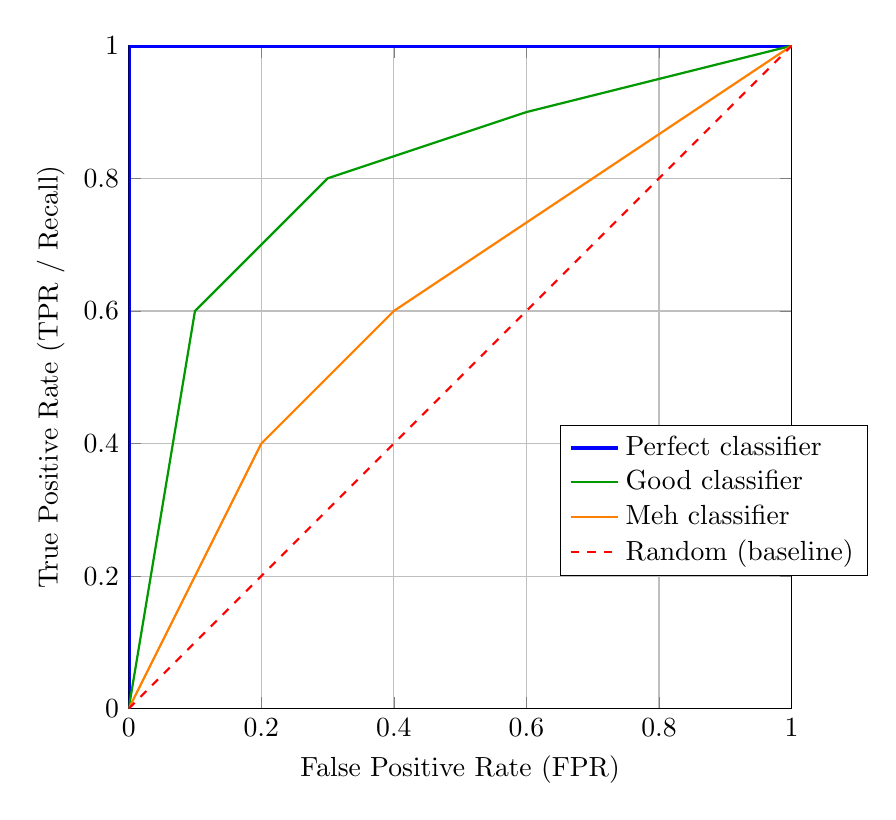
\begin{tikzpicture}
\begin{axis}[
    width=10cm,
    height=10cm,
    xlabel={False Positive Rate (FPR)},
    ylabel={True Positive Rate (TPR / Recall)},
    xmin=0, xmax=1,
    ymin=0, ymax=1,
    grid=both,
    legend style={at={(0.65,0.2)}, anchor=south west},
    legend cell align={left},
]

% Perfect classifier
\addplot[
    ultra thick,
    blue
]
coordinates {
    (0,0)
    (0,1)
    (1,1)
};
\addlegendentry{Perfect classifier}

% Good classifier
\addplot[
    thick,
    green!60!black
]
coordinates {
    (0,0)
    (0.1,0.6)
    (0.3,0.8)
    (0.6,0.9)
    (1,1)
};
\addlegendentry{Good classifier}

% Meh classifier
\addplot[
    thick,
    orange
]
coordinates {
    (0,0)
    (0.2,0.4)
    (0.4,0.6)
    (0.7,0.8)
    (1,1)
};
\addlegendentry{Meh classifier}

% Random classifier
\addplot[
    thick,
    dashed,
    red
]
coordinates {
    (0,0)
    (1,1)
};
\addlegendentry{Random (baseline)}

\end{axis}
\end{tikzpicture}


\vspace{10pt}

Another useful curve is the \textbf{Precision-Recall Curve}. We can find the best threshold for the F1 maximization.

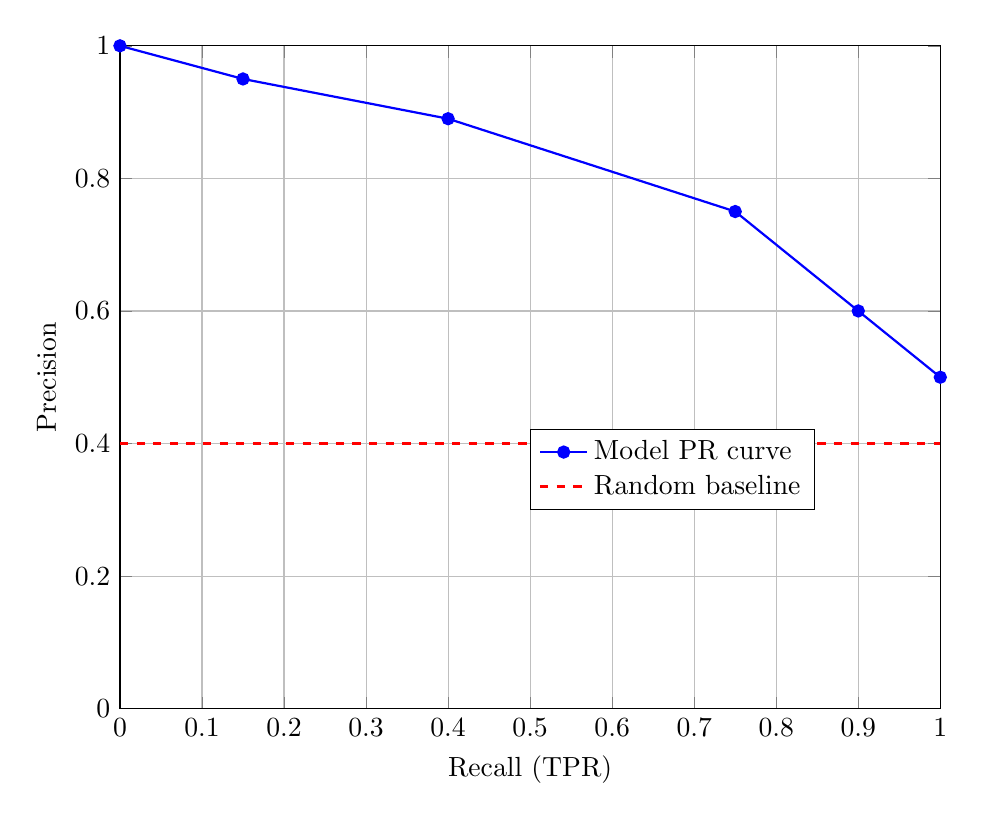
\begin{tikzpicture}
\begin{axis}[
    width=12cm,
    height=10cm,
    xlabel={Recall (TPR)},
    ylabel={Precision},
    xmin=0, xmax=1,
    ymin=0, ymax=1,
    grid=both,
    legend style={at={(0.5,0.3)}, anchor=south west},
    legend cell align={left},
]

% Realistic PR curve
\addplot[
    thick,
    blue,
    mark=*,
]
coordinates {
    (0.0, 1.0)
    (0.15, 0.95)
    (0.40, 0.89)
    (0.75, 0.75)
    (0.90, 0.60)
    (1.0, 0.50)
};
\addlegendentry{Model PR curve}

% Random baseline (precision = prevalence)
\addplot[
    thick,
    dashed,
    red
]
coordinates {
    (0,0.4)
    (1,0.4)
};
\addlegendentry{Random baseline}

\end{axis}
\end{tikzpicture}


\vspace{20pt}

For regression tasks we can use the following metrics

\begin{itemize}

  \item \textbf{Mean Absolute Error (MAE)} \\
  $\displaystyle \text{MAE} = \frac{1}{n} \sum_{i=1}^{n} |y_i - \hat{y}_i|$

  \item \textbf{Mean Squared Error (MSE)} \\
  $\displaystyle \text{MSE} = \frac{1}{n} \sum_{i=1}^{n} (y_i - \hat{y}_i)^2$

  \item \textbf{Coefficient of Determination ($R^2$)} \\
  $\displaystyle R^2 = 1 - \frac{\sum_{i=1}^{n} (y_i - \hat{y}_i)^2}{\sum_{i=1}^{n} (y_i - \bar{y})^2}$

  \item \textbf{Adjusted $R^2$} \\
  $\displaystyle R^2_{\text{adj}} = 1 - \left(1-R^2\right)\frac{n-1}{n-p-1}$

\end{itemize}

\vspace{10pt}

Remember that

\begin{itemize}
    \item MSE and RMSE penalize large errors
    \item If we don't care use MAE
    \item If we have different numbers of predictors use Adjusted $R^2$
\end{itemize}



\subsection{Bayesians classifiers}

Bayesian classifiers are a class of probabilistic classifers, they give probabilities of
being part of a certain class with respect to another.
The reasons that we use them are:
\begin{itemize}
    \item They are statistical
    \item Based on Bayes theorem
    \item They have very good performance
    \item They are incremental
    \item They set a standard of quality
\end{itemize}

\vspace{10pt}

Recall Bayes theorem

\begin{equation}
    P(H|E) =  \frac{P(H)P(E|H)}{P(E)}
\end{equation}

Where:

\begin{itemize}
    \item H is our hypothesis
    \item E is an evidence of the hypothesis
\end{itemize}

We can update both E and H with new knowledge.

\vspace{10pt}

If we assume E to be a data sample with attributes and an unknown class label and H
to be an hypothesis that E belongs to a class C and we want to determine P(H|E) with 
the Bayes theorem we get
\begin{equation}
    \text{Posterior} = \frac{\text{Likelihood * Prior}}{\text{Evidence}}
\end{equation}

Basically

\begin{itemize}
    \item Likelihood \ra The probability of observing the sample given that the hypothesis is true
    \item Prior \ra Probability that a certain event happens regardless of the evidence
    \item Evidence \ra Probability that our sample is observed
\end{itemize}

We can either maximise the likelihood or the posterior

\vspace{10pt}

Maximising the posterior means maximising:

\begin{equation}
    P(C_i|X) = P(X|C_i)P(C_i)
\end{equation}

\vspace{10pt}

A special case is the Naive Bayes Classifier where we assume that P(X) is equal for all the classes.
So the attributes are conditionally independent.
To avoid that the probabilities of events without occurence in our sample will be zero we add one occurence to every value class combination (Laplace estimator).
In case of missing values the instance is not included in the frequency counts during training, while for classification the attribute will be omitted from calculation

\vspace{10pt}

Knowing that the probability density function of a normal distribution is based on the two paramenters mean and standard deviation we can
use those information in the sample to estimate the probabilities

\vspace{10pt}

Naive Bayes can have good sides

\begin{itemize}
    \item Easy to implement
    \item Good results
\end{itemize}

\vspace{10pt}

But also cons 
\begin{itemize}
    \item We lose accuracy assuming class independency
    \item Dependencies exist in real life 
\end{itemize}

To solve the cons we use \textbf{Bayesians Belief Networks}. They allow for class conditional independencies between subsets of variables.
Those networks are composed by two components
\begin{enumerate}
    \item Directed acyclic graph \ra Shows dependency among the variables and gives specification of joint probability distribution.
    \item Set of conditional probabilities
\end{enumerate}

The nodes of the graph represent the variables while the arcs are the dependencies among the variables.
The relationship among the variables \ra Each variable is conditionally independent of its non descendants in the network given the parennts.



\subsection{Instance based learning}

Instance based classifiers use the simplest form of learning, we just compare previous
seen examples and we classifiy the new instance by similarity. We call this approach lazy learning. Some important concepts are
feature space and similarity measures. The most basic algorithm is the nearest-neighbor that can be extended to KNN and K-d Trees.
The simplest idea is that we store the training records and we use them to predict the class label of unseen cases.
If we don't find an exact match we just use the closest point. Since using just one point would have too high of an impact with outliers we 
dilute the depencdency on individual points and we use the k closest ones. 

\vspace{10pt}

As said we can use KNN, it requires 3 things:
\begin{itemize}
    \item The set of stored records
    \item Distance metric to compute the distance between records
    \item The number k
\end{itemize}

With K equal to 1 we can get a Voronoi diagram, we plot a decision boundary. 

\vspace{10pt}

Another thing that we have to decide is the choice of the distance metric.

The most used are

\begin{itemize}
    \item \textbf{Euclidean:}
    \[
        d_E(x, y) = \sqrt{\sum_{i=1}^{n} (x_i - y_i)^2}
    \]

    \item \textbf{Manhattan:}
    \[
        d_M(x, y) = \sum_{i=1}^{n} |x_i - y_i|
    \]

    \item \textbf{Minkowski:}
    \[
        d_p(x, y) = \left( \sum_{i=1}^{n} |x_i - y_i|^p \right)^{\frac{1}{p}}
    \]
\end{itemize}

To determine the class we can either take a vote of class labels among the K nearest neighbors or vote according to the distance using the 
reciprocal squared distance

\[
w = \frac{1}{d^2}
\]

\vspace{10pt}

One variant of the KNN is the distance-Weighted KNN where nearer neighbours will have more weight in the vote

\begin{equation*}
    f(\mathbf{X}_q) = \frac{\displaystyle\sum_{i=1}^{k} w_i\, f(\mathbf{X}_i)}{\displaystyle\sum_{i=1}^{k} w_i} \text{where} w_i = \frac{1}{d(\textbf{X}_q, \textbf{X}_i)^2}
\end{equation*}

With this approach called Stepard method we can use all the training examples.

\vspace{10pt}

Another critical aspect is the choice of the optimal k, if its too small we risk overfit and will be too sensitive to noisy points. If k is too large we might not find the true pattern of the data and we risk underfitting.
For a balanced dataset our decision boundary will resemble a linear regression, k\ra n

\vspace{10pt}

Since is a scale sensitive algorithm we have to normalize the features to prevent one measure to dominate on the others.

We need to put caution for irrelevant attributes. Also calculating the distances can be computationally expensive. KNN algorith are sensitive to outliers and to the choice of the distance.

\vspace{10pt}

To solve the problem of calculating all distances we can create an index of the distances to retrieve the neighbors efficiently. We get a k-d tree. A k-d tree is a balanced binary tree where each node indexes one of the instances of the training set.

The get a K-d tree

\begin{enumerate}
    \item Make a list of the features in a randomized order
    \item Find the meadian of the first feature and split the data
    \item Split untill we have less than 2 datapoints in each node.
\end{enumerate}

To find the nearest neighbor, we traverse the tree from the leaves upward.
At each step, we calculate the distance between the query point and the current node, then compare it with the distance to the parent node.
We always keep the node with the smallest distance.
At each branching point, we check which branch gives the smaller distance and continue this process until we reach the root.
The nearest neighbor is the node with the smallest overall distance.

K-d trees are useful when we have many more instances than features. We can also adappt them to predict continuous target ussing the average of the nearest neighbors.

Othe similarity measures that can be used are
\begin{enumerate}
    \item Co-presence
    \item Co-absence
    \item Presence-absence
    \item Absence-presence
    \item Russel Rao similarity index \ra uses only CP
    \item Sokal-Michener similarity index \ra Uses CP and CA
    \item Jaccard similarity index \ra uses all but CA
    \item Cosine similarity
    \item Mahalanobis distance
\end{enumerate}

\subsection{Neural Networks}

One new family of algorithm is the ones of the neural networks. They have many applications in many fields and like
AI they had periods of summers and winters. The strength of neural networks comes from
the fact that they learn automatically, are data driven and can be universal approximators also
for non linear problems. Even though they are pretty much two completely different things 
neural networks are inspired by biological brain structures. The idea is that neurons will fire after they recieve 
a certain input and so will our perceptrons after their activation fucntion manages to go over a certain threshold.

\vspace{10 pt}

Neural networks receive some inputs x from other neurons or the environment and will feed an output to a connection with a certain weight that will go to the next neuron.
The total input that a neuron receives is the weighted sum of inputs from all the sources. The activation function will make the output from the input.

A neural network usually with one neuron (perceptron) has 4 elements

\begin{itemize}
    \item Input 
    \item Weights
    \item Bias
    \item Activation function
\end{itemize}

The activation function can be of 3 kind

\begin{itemize}
    \item Tanh
    \item Sigmoid
    \item Threshold model (can be Relu or the identity)
\end{itemize}

As said the models will learn automatically by adjusting the weights in the network to reach as much generalization as possible.
The idea is like trial and error
\begin{enumerate}
    \item Random weights
    \item Small adjustments until we reach a good result
\end{enumerate}

We have two main kind of signals: the function (input to output) and the error (output to input).

After we calculate the error we go back to change a bit the weights every time we iterate with the model.

\vspace{10pt}

The model will generate an hyperplane to divide the dataset into the classes (if classification).
For linear problems we can use just one perceptron (will converge after enough iterations) while for non linear ones we might need more layers. 

\vspace{10pt}
With more layers we enter the domain of the \textbf{Multilayer Perceptron (MLP)}.

\begin{itemize}
    \item \textbf{Input layer} $\rightarrow$ Each neuron receives one input from the outside.
    \item \textbf{Hidden layer(s)} $\rightarrow$ Connect the input layer to the output layer; usually one or two hidden layers are enough.
    \item \textbf{Output layer} $\rightarrow$ Produces the final prediction.
\end{itemize}

The training algorithm is called \textbf{Backpropagation}.  
We define a loss function (which measures the error) and we want to minimize it.  
This is done by computing its gradient with respect to the weights.

The variation of the loss for different weight values defines the \textbf{error surface},  
while the difference between the network output and the target defines the \textbf{error signal}.
\vspace{10pt}
Delta rule (error term)

For a unit $j$ in the \textbf{output layer}:
\[
\mathrm{Err}_j = O_j (1 - O_j)\,(T_j - O_j)
\]

For a unit $j$ in a \textbf{hidden layer}:
\[
\mathrm{Err}_j = O_j (1 - O_j)\sum_{k} \mathrm{Err}_k \, w_{jk}
\]
\vspace{10pt}
Weight update rule

For a weight $w_{ij}$ connecting neuron $i$ to neuron $j$:

\[
\Delta w_{ij} = \alpha\, \mathrm{Err}_j \, a_i
\]

where $\alpha$ is the learning rate and $a_i$ is the activation of neuron $i$.

The weight update becomes:

\[
w_{ij}^{\text{new}} = w_{ij}^{\text{old}} + \Delta w_{ij}
\]

or equivalently:

\[
w_{ij} = w_{ij}^{\text{old}} + \alpha\, \mathrm{Err}_j \, a_i.
\]


\subsection{Decision Trees}

The class of decision trees can be applied both at classification and estimation. A good advantage is that the trees represent rules, so we can interpret the results very well. 

\vspace{10pt}

At each level we set a rule and we divide our sample in different branches, we will do that untill we will reach a certain granularity in our results. Our test set data will flow in the tree and we will get a solution based on where they fall. If we want to discriminate between classes we want to have leaves that are as pure as possible, so that they represent only individuals of a particular class. 

Each edge will add a conjunction and each new leaf will add a disjunction.

\vspace{10pt}

As said decision trees have many advantages

\begin{itemize}
    \item Interpretability
    \item Can deal with different types of data
    \item Don't care about scale of the data
    \item Automatic definition of the useful attributes for each class
    \item Can be used for regression
    \item Non-parametric
\end{itemize}

But also disadvantages

\begin{itemize}
    \item Most algorithms will require a discrete target
    \item Small data variations can result in different trees
    \item Sub-trees can be duplicated several times
    \item With many classes we have worse results
    \item Linear boundaires should be perpendicular to the axis
\end{itemize}


When we bulid a decision tree we start from our training set and we have to decide 

\begin{itemize}
    \item Which variable to query 
    \item Where to cut
    \item Which node we should part
    \item How many edges per node
    \item When to stop
\end{itemize}

At each level we can divide an independet variable into different partitions where we want to measure the evaluate the quality of it. We do that continuously untill we don't reach the stopping criterion. 

\vspace{10pt}

The algorithm is a greedy one

\begin{itemize}
    \item The tree is built in a top-down recursive divide-and-conquer manner
    \item All training examples start at root
    \item If the attributes that are selected are continuous they are discretized
    \item Examples are partitioned based on the selected attributes
    \item Test attributes are selected on the basis of a heuristic or statistical measure
\end{itemize}

On the other hand to stop the partitions

\begin{itemize}
    \item All samples in a node belongs to the same class
    \item We can't divide anymore and we use majority voting to classify
    \item There are no samples left
\end{itemize}

Also we can have different algorithms

\begin{itemize}
    \item DDT 
    \item ID3, C4.5, C5
    \item CART
    \item CHAID
    \item And many more
\end{itemize}

More specifically

\vspace{10pt}

\textbf{DDT}
\begin{itemize}
    \item Greed search
    \item No backtraking
    \item Can be stuck in a local minimum
    \item We start with a dataset o pre-classified individuals and each node specifies an attribute used as a test
    \item The metric is a discriminative one $f(a) = \frac{1}{n} \sum_{i=1}^{|A|} C_i$ to measure the dominance or purity of the most frequent class
    
\end{itemize}

\vspace{10pt}

\textbf{ID3, C4.5}
\begin{itemize}
    \item We select the attribute with the highest information gain
    \item So we want to minimize the entropy $Entropy(D) = - \sum_{i=1}^{m} p_i log_2(p_i)$
    \item If we choose the attribute A to split the node with the tuples in D in v partitions the information needed to classify D is $ Entropy_A(D) = \sum_{j=i}^{y} \frac{|D_j|}{|D|} \times Entropy(D_j)$
    \item The information gained by branching on attribute A is $ Gain(A) = Entropy(D) - Entropy_A(D)$
\end{itemize}


\vspace{10pt}
\textbf{CART}

\begin{itemize}
    \item We use the Gini index $gini(D) = 1 - \sum_{j=1}^{n}p^2_j$
    \item If a data set D is split on A in D1 and D2 the gini index is $ gini_{age}(D) = \frac{|D_1|}{|D|} gini(D_1) + \frac{|D_2|}{|D|}gini(D_2)$
    \item We have a reduction in impurity $\Delta gini(A) = gini(D) - gini_A(D)$
    \item We choose the attribute that maximises the reduction in impurity
\end{itemize}

\vspace{10pt}

One problem of trees is that they are very prone to overfit on the training data. To solve we can either do

\begin{itemize}
    \item Prepruning \ra We will not split a node if the goodness of the measure will go under a threshold
    \item Postpruning \ra We remove leaves and branches after the tree is made
\end{itemize}

\vspace{10pt}

Trees can also be used for regression tasks. Every leaf represents a value and we will predict that value (or mean of several values) if our instance is falling in the designated area of our tree.

To find the best splitting point of a tree we can use the MSE and minimize the local split errors. We can also use MAE or sum of residuals.
MSE at the leaf level will use the mean value while MAE will go with the median. 
But the important thing is to determine a stopping point since we can easily overfit if we have one leaf for every possible value.

\vspace{10pt}

Since we want to avoid overfit we can do that by removing a leaf, calculate the MSE and do that for everyone. We will stay with the best tree.

This can be problematic since every time we remove a leaf the MSE will grow, then we use the Tree score

\[
TressScore = MSE + \alpha T
\]

$\alpha$ is an hyperparameter that we find using our validation set, T is the number of leaves.

\begin{enumerate}
    \item Compute the cost complexity pruning path by creating a fully grown tree and compute the $\alpha$ that minimizes the TreeScore.
    \item Split the data for cross validation
    \item For each $\alpha$ prune the tree
    \item Find the average validation score
    \item Select the optimal $\alpha$
    \item Train the final model
\end{enumerate}

\subsection{Ensemble Learning}

Ensemble Learning means combinining multiple models to achieve better performance than any single one. It can overcome problems like overfitting, being stuck in local optima and expanding the space of representable functions. Based on the idea of "The wisdom of crowds". The google search algorithm is an ensemble. 

\vspace{10pt}

Theoretical and empirical studies demonstrated that ensembles are tipically more accurate than single classifiers. Though we don't have a single and rigourous definiton of ensembled classifiers. We can see neural networks as ensembles and see that they can be seen as universal approximators with this idea.

\vspace{10pt}

Ensembles work from the Bias-Variance decomposition

\[
\text{Expected Prediction Error} = \text{Bias}^2 + Variance + Irreducible Error
\]

\begin{itemize}
    \item Bagging reduces variance
    \item Boosting reduces bias
    \item Stacking reduces both
\end{itemize}


Classifier ensembles work due to

\begin{itemize}
    \item Statistical reasons \ra Since we are observing a large searching space we might not find the global optimum so we can average several local ones to get a solid solution
    \item Computational reasons \ra Can be given by imperfect training algorithms, too much data, small sample size, divide and conquer solutions and data fusion
\end{itemize}

\includegraphics[width=17cm]{ensemble tree.png}

\textbf{How to set up an ensemble}

\begin{itemize}
    \item Combination Level
    \begin{itemize}
        \item How are the individual inputs combined?
    \end{itemize}

    \item Classifier Level
    \begin{itemize}
        \item Do we use same or different classifiers?
        \item What base classifier is best: decision tree, NN or another?
        \item How many classifiers are needed? Do we overproduce and select?
        \item Should the $L$ classifiers be trained together or incrementally?
    \end{itemize}

    \item Feature Level
    \begin{itemize}
        \item Shall we use all features or use a bespoke subset for each classifier?
        \item How do we select/extract such subsets?
    \end{itemize}

    \item Data Level
    \begin{itemize}
        \item How can we manipulate the data submitted for training to the base classifier so as to ensure high diversity and high individual accuracy?
    \end{itemize}
\end{itemize}

\vspace{10pt}

\begin{itemize}
    \item A combiner can be
    \begin{itemize}
        \item Nontrainable
        \item Trainable
        \item Meta classifier
    \end{itemize}

    \item To build the ensemble
    \begin{itemize}
        \item The classifiers can be trained independently or in sequence
    \end{itemize}

    \item How to introduce diversity
    \begin{itemize}
        \item Use different approaches and parameters
        \item Manipulate the training samples
        \item Use different target labels
        \item Partition the dataset
        \item Use different classifier models or hybrid ensembles
    \end{itemize}

    \item Ensemble size
    \begin{itemize}
        \item Determine the number of classifiers in the ensemble
    \end{itemize}

    \item Universality
    \begin{itemize}
        \item Some approaches can be used with any classifier while others are specifically for a subset of them, like the random forest
    \end{itemize}
\end{itemize}

\vspace{10pt}

Ensemble learning has some benefits

\begin{itemize}
    \item Improved accuracy
    \item Less overfitting
    \item Increased robustness
    \item Versatility
    \item Handling of complex problems
    \item Bias reduction
    \item Imbalanced data performance
\end{itemize}

We have two main strategies
\begin{itemize}
    \item Fusion \ra each ensemble member knows the whole feature space
    \item Selection \ra each member knows a subset of the space in a specialized way
\end{itemize}


The outputs can be of three levels

\begin{enumerate}
    \item Abstract \ra each member output one prediction
    \item Ranked \ra each member ranks the predictions in order of plausability
    \item Measurement \ra each classifer outputs the confidence for each prediction
\end{enumerate}

The final output is usually given by a majority voting choosing the class that has been selected the majority of the times. By Condorcet Jury Theorem as the number of classifiers L \ra $\infty$ the ensemble accuracy $P_maj$ \ra 1.0.

\vspace{10pt}

If we consider that the classifiers have different accuracy level we can use a weighted majority vote with some parameters that will sum to 1. 

\vspace{10pt}

For regression the final output can be obtained by averaging the predictions of the others. 

\vspace{10pt}

Specifically of meta-algorithms we have the idea pf ensemble methods, they combine several machine learning techniques in one predictive model to

\begin{itemize}
    \item Decrease variance \ra Bagging
    \item Decrease bias \ra Boosting
    \item Improve predictions \ra Stacking
\end{itemize}

\vspace{10pt}

\textbf{Bagging} \ra acronym for Bootstrap AGGregatING, the ensemble is built on bootstrap replicates of the training set and the outputs are combined by plurality vote. We obtain diversity by using different training sets. The base classifier should be unstable, small changes will have to lead to large ones. Usually 25 to 30 decision trees are sufficient. If the classifiers are independent we are guaranteed an improve on the individual performance. The idea of bootstrapping is to randomly drawing with replacement B observations from our dataset and train on them.

\vspace{10pt}

The most famous algorithm is the Random forest. Is a very efficient algorithm on large data sets. The randomness is given by choosing a random training set for each base learner and the fact that the splits of the decision trees are chosen randomly.

\begin{itemize}
    \item From the training set, create $t$ bootstrap samples
    \begin{itemize}
        \item Similar to Bagging, but generally the size of bootstrap samples is the same as the size of the training set
    \end{itemize}

    \item Attribute selection
    \begin{itemize}
        \item If there are a total of $X$ attributes in the observations, choose a number $x \ll X$, e.g., $x = \sqrt{X}$
        \item This value of $x$ is held constant while growing the forest
        \item For the split of each node in each base learner (Decision Tree), randomly select $x$ attributes out of $X$
        \item Choose one attribute out of $x$ to split the node
        \item This is one reason Random Forest trees are created faster than regular trees, where each split decision involves all attributes
    \end{itemize}

    \item Tree growth
    \begin{itemize}
        \item Each tree is grown to the largest extent possible
        \item No pruning, since we desire high variance and low correlation between any two base learners
    \end{itemize}

    \item Steps summary
    \begin{enumerate}
        \item Bootstrap data
        \item Randomly select attributes for each node
        \item Build tree until end
        \item Calculate performance from OOB (Out-Of-Bag) observations
    \end{enumerate}
\end{itemize}


\subsection{SVM}

Support vector machines are a supervised ML algorithm that can be used for classification and regression. Like for KNR we plot the points obtaining the coordinates but we try to create an hyperplane that maximises the difference between the different classes. The border is defined by the points nearest to them, those are our support vectors. The hyperplane is linear. 

\vspace{10pt}

With previous approach every line that splits the classes are ok, here we aim at find the "best one", where the space between the border points is maximised. This idea can also be called widest street approach. 

Imagine a vector $\mathbf{w}$ of any length and perpendicular to the median line (dashed line).
Now imagine an unknown point, and a vector pointing to it $\mathbf{u}$.
What we would like to know is whether $\mathbf{u}$ is on the left or on the right side of the street.

\bigskip


\includegraphics[width=5cm]{svm.png}

So, we project the vector $\mathbf{u}$ onto $\mathbf{w}$ (which is perpendicular to the street) and measure whether
\[
\mathbf{w} \cdot \mathbf{u} \ge c
\]
or equivalently
\[
\mathbf{w} \cdot \mathbf{u} + b \ge 0,
\]
with $c = -b$.

In this case, the event is classified as positive.


The decision rule of an SVM classifier is:
\[
\mathbf{w} \cdot \mathbf{u} + b \ge 0
\]

However:
\begin{itemize}
\item we do not know $b$,
\item we do not know $\mathbf{w}$,
\item there are infinitely many vectors $\mathbf{w}$ perpendicular to the separating hyperplane.
\end{itemize}

Therefore, we need additional constraints to determine $\mathbf{w}$ and $b$.



By introducing constraints, we assume:
\[
\mathbf{w} \cdot \mathbf{x}^+ + b \ge 1
\]
\[
\mathbf{w} \cdot \mathbf{x}^- + b \le -1
\]

This imposes a separation from $-1$ to $+1$ for all known samples.
We can now solve the system to find $\mathbf{w}$ and $b$ that guarantee this separation for all training samples.


For convenience, we introduce labels $y_i$ such that:
\[
y_i =
\begin{cases}
+1 & \text{for positive samples} \\
-1 & \text{for negative samples}
\end{cases}
\]

Multiplying the constraints by $y_i$, we obtain:
\[
y_i \left( \mathbf{w} \cdot \mathbf{x}_i + b \right) \ge 1
\]

This can be rewritten as:
\[
y_i \left( \mathbf{w} \cdot \mathbf{x}_i + b \right) - 1 \ge 0
\]


For samples lying exactly on the margin (support vectors), the constraint becomes:
\[
y_i \left( \mathbf{w} \cdot \mathbf{x}_i + b \right) - 1 = 0
\]


These constraints define the two boundaries of the street such that the separation between positive and negative examples is as wide as possible.


Consider one positive sample $\mathbf{x}^+$ and one negative sample $\mathbf{x}^-$.
Their difference is:
\[
\mathbf{x}^+ - \mathbf{x}^-
\]

The width of the margin is obtained by projecting this difference onto the unit vector normal to the hyperplane.
Since $\mathbf{w}$ is normal to the median line, its unit vector is:
\[
\frac{\mathbf{w}}{\|\mathbf{w}\|}
\]

Thus, the width of the street is:
\[
\text{width} = (\mathbf{x}^+ - \mathbf{x}^-) \cdot \frac{\mathbf{w}}{\|\mathbf{w}\|}
\]


From the boundary condition:
\[
y_i \left( \mathbf{w} \cdot \mathbf{x}_i + b \right) - 1 = 0
\]

we obtain:
\[
\mathbf{w} \cdot \mathbf{x}_i = 1 - b \quad \text{for positive samples}
\]
\[
\mathbf{w} \cdot \mathbf{x}_i = -1 - b \quad \text{for negative samples}
\]

Therefore:
\[
\text{width} =
\frac{\mathbf{x}^+ \cdot \mathbf{w} - \mathbf{x}^- \cdot \mathbf{w}}{\|\mathbf{w}\|}
=
\frac{(1 - b) - (-1 - b)}{\|\mathbf{w}\|}
=
\frac{2}{\|\mathbf{w}\|}
\]


To maximize the margin width:
\[
\frac{2}{\|\mathbf{w}\|}
\]

it is sufficient to minimize $\|\mathbf{w}\|$.
For mathematical convenience, this is usually formulated as minimizing:
\[
\frac{1}{2} \|\mathbf{w}\|^2
\]

From Calcus 2, to minimize a function on a constrained domain we can use the Lagrange multipliers method

Assume that $L$ (the Lagrangian) is the function that we want to minimize:
\[
L = \frac{1}{2}\|\mathbf{w}\|^2 - \sum_i \alpha_i \left[ y_i (\mathbf{w} \cdot \mathbf{x}_i + b) - 1 \right]
\]

We subtract the sum of all constraints multiplied by constants $\alpha_i$ (one for each constraint).

Finding an extremum implies computing the derivatives and setting them equal to zero.



\[
\frac{\partial L}{\partial \mathbf{w}} = \mathbf{w} - \sum_i \alpha_i y_i \mathbf{x}_i = 0
\]

which implies:
\[
\mathbf{w} = \sum_i \alpha_i y_i \mathbf{x}_i
\]

Therefore, $\mathbf{w}$ is a linear combination of the vectors in the training set.


The Lagrangian must be differentiated with respect to all variables that may vary, including $b$:
\[
\frac{\partial L}{\partial b} = - \sum_i \alpha_i y_i = 0
\]

which implies:
\[
\sum_i \alpha_i y_i = 0
\]


Recall the expression for the decision vector:
\[
\mathbf{w} = \sum_i \alpha_i y_i \mathbf{x}_i
\]

We now substitute $\mathbf{w}$ into the Lagrangian:
\[
L =
\frac{1}{2}
\left(
\sum_i \alpha_i y_i \mathbf{x}_i
\right)
\cdot
\left(
\sum_j \alpha_j y_j \mathbf{x}_j
\right)
-
\sum_i \alpha_i y_i \mathbf{x}_i
\cdot
\left(
\sum_j \alpha_j y_j \mathbf{x}_j
\right)
-
\sum_i \alpha_i y_i b
+
\sum_i \alpha_i
\]

Since $b$ is a constant and
\[
\sum_i \alpha_i y_i = 0,
\]
we have:
\[
\sum_i \alpha_i y_i b = b \sum_i \alpha_i y_i = 0
\]

Thus, the Lagrangian can be rewritten as:
\[
L =
\frac{1}{2}
\sum_i \alpha_i y_i \mathbf{x}_i
\cdot
\sum_j \alpha_j y_j \mathbf{x}_j
-
\sum_i \alpha_i y_i \mathbf{x}_i
\cdot
\sum_j \alpha_j y_j \mathbf{x}_j
+
\sum_i \alpha_i
\]

which simplifies to:
\[
L =
\sum_i \alpha_i
-
\frac{1}{2}
\sum_i
\sum_j
\alpha_i \alpha_j y_i y_j
(\mathbf{x}_i \cdot \mathbf{x}_j)
\]


We find that the optimization depends only on the dot product of pairs of samples.


Recall the decision rule for a new observation $\mathbf{u}$:
\[
\mathbf{w} \cdot \mathbf{u} + b \ge 0
\]

Substituting $\mathbf{w}$, we obtain:
\[
\left( \sum_i \alpha_i y_i \mathbf{x}_i \right) \cdot \mathbf{u} + b \ge 0
\]

If the inequality holds, the sample is classified as positive.

Only points lying on the margin (i.e.\ the support vectors $\mathbf{x}_i$) have $\alpha_i > 0$.

Therefore, the decision rule depends only on the dot product between training samples and the unknown observation.


It can be shown (proof omitted) that this optimization problem is convex.
This implies that there are no local minima.

As a consequence, any reasonable optimization algorithm (including Hill Climbing) can find the global optimum (or a very good approximation of it).


% Primo vettore: parametri del modello (w1, w2, b)
\[
\begin{pmatrix}
w_1 \\
w_2 \\
b
\end{pmatrix}
=
\begin{pmatrix}
-0.4615 \\
-0.3076 \\
-3.6153
\end{pmatrix}
\]

% Secondo vettore: moltiplicatori di Lagrange (alpha1, alpha2, alpha3)
\[
\begin{pmatrix}
\alpha_1 \\
\alpha_2 \\
\alpha_3
\end{pmatrix}
=
\begin{pmatrix}
0.1538 \\
0 \\
0.1538
\end{pmatrix}
\]
% Interpretation of points and SVM parameters

Consider the vector of Lagrange multipliers:
\[
\alpha = 
\begin{pmatrix} 0.1538 \\ 0 \\ 0.1538 \end{pmatrix}
\]

Quick interpretation:
\begin{itemize}
    \item $\alpha_i > 0$: the point is a \textbf{support vector} and contributes to the decision boundary.
    \item $\alpha_i = 0$: the point does not contribute, it is ignored.
\end{itemize}

For example, here points 1 and 3 are support vectors, point 2 does not influence the model.

---

The decision parameters are given by:
\[
\mathbf{w} = 
\begin{pmatrix} w_1 \\ w_2 \end{pmatrix} =
\begin{pmatrix} -0.4615 \\ -0.3076 \end{pmatrix}, 
\quad b = -3.6153
\]

- $w_1, w_2$ determine the \textbf{slope} of the decision line.
- $b$ shifts the line up or down without changing its slope.

The equation of the decision boundary is:
\[
w_1 x_1 + w_2 x_2 + b = 0 \quad \text{or equivalently} \quad x_2 = -\frac{w_1}{w_2} x_1 - \frac{b}{w_2}
\]

---

To classify a new point $\mathbf{u} = (u_1, u_2)$:
\[
\text{score} = w_1 u_1 + w_2 u_2 + b
\]

- score $> 0$ $\Rightarrow$ positive side
- score $< 0$ $\Rightarrow$ negative side
- score $\approx 0$ $\Rightarrow$ near the margin

---

Summary (at a glance):
\begin{itemize}
    \item Check $\alpha_i$ to identify support vectors.
    \item Use $\mathbf{w}$ and $b$ to define the line slope and position.
    \item Evaluate $w \cdot u + b$ for a new point to see which side it falls on.
\end{itemize}

The main parameter of SVM is C, we can choose the trade-off between error and margin. C is adjusted by the user. Large C means high penalty to classification errors, the number of missclassified patterns is minimized. With smaller C the points go inside the margin. 

\vspace{10pt}

If we have inseparable data we can project them into an higher feature space (like from 1 to 2 dimensions) to make them separable. Those functions are called kernel

Some examples are

\begin{itemize}
    \item Polynomial
    \item Radial
    \item Sigmoid
\end{itemize}

% Explanation of gamma in RBF kernel

Gamma ($\gamma$) is the free parameter of the Gaussian radial basis function (RBF).

\begin{itemize}
    \item \textbf{Small gamma:} The Gaussian has a large variance.  
    This means each support vector influences a \textbf{large area} around itself.  
    Even points that are far away from the support vector are affected, making the model smoother and more general.
    
    \item \textbf{Large gamma:} The Gaussian has a small variance.  
    Each support vector influences only points very close to it.  
    Points farther away are hardly affected, making the model more sensitive to the training points (risking overfitting).
\end{itemize}

\textbf{Analogy:} Imagine a bell above each support vector:
\begin{itemize}
    \item Small gamma $\rightarrow$ wide bell $\rightarrow$ many points hear it
    \item Large gamma $\rightarrow$ narrow bell $\rightarrow$ only nearby points hear it
\end{itemize}
